\begin{titlepage}
    \centering
    
    \vspace*{1cm}
    
    \Huge\textsf{\textbf{Software Verification}}
    
    \vspace{0.5cm}
%   \LARGE\textsf{- A Deep Dive into Testing and Validation -}
    \LARGE\textsf{- Logic-based Program Verification -}
    
    \vspace{1.5cm}
    \textbf{Ji, Yong-Hyeon}

	\vspace{2cm}
%	\begin{figure}[h!]\centering
%	\begin{tikzpicture}
%		% Set colors for different logics
%		\definecolor{plcolor}{RGB}{255, 204, 204}
%		\definecolor{folcolor}{RGB}{204, 229, 255}
%		\definecolor{holcolor}{RGB}{204, 255, 204}
%		
%		% Draw the Higher-Order Logic (HOL) circle
%		\fill[holcolor] (0,0) circle (6cm);
%		\draw (0,0) circle (6cm);
%		\node at (0, 5.25) {\bf Higher-Order Logic (HOL)};
%		
%		% Draw the First-Order Logic (FOL) circle
%		\fill[folcolor] (0,0) circle (5cm);
%		\draw (0,0) circle (5cm);
%		\node at (0, 3.75) {\bf First-Order Logic (FOL)};
%		
%		% Draw the Propositional Logic (PL) circle
%		\fill[plcolor] (0,0) circle (3cm);
%		\draw (0,0) circle (3cm);
%		\node at (0, 0) {\bf Propositional Logic (PL)};
%		
%	\end{tikzpicture}
%	\end{figure}
	\begin{center}
	\adjustbox{scale=.9}{
	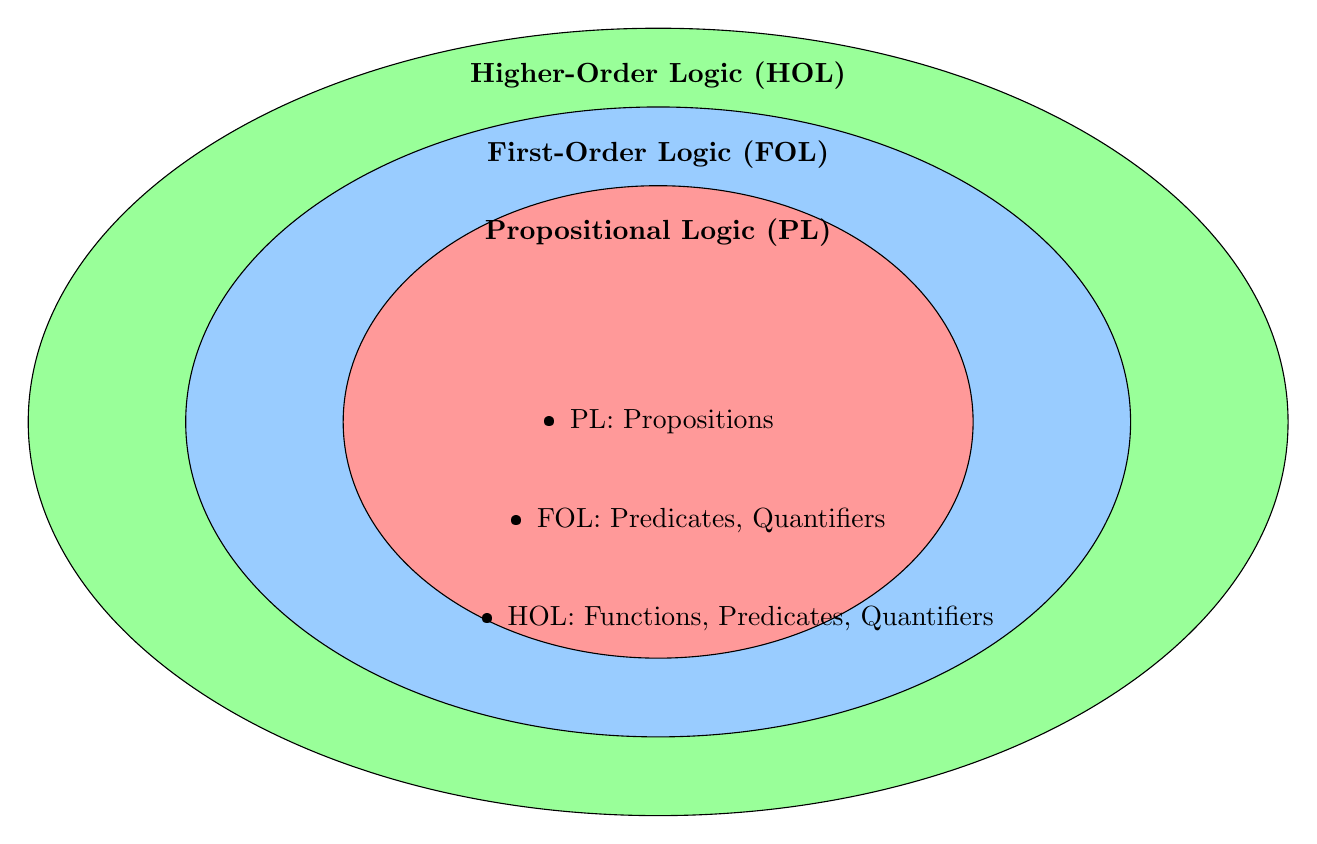
\begin{tikzpicture}
		
		% Define colors
		\definecolor{plcolor}{RGB}{255, 153, 153}
		\definecolor{folcolor}{RGB}{153, 204, 255}
		\definecolor{holcolor}{RGB}{153, 255, 153}
		
		% Draw the Higher-Order Logic (HOL) ellipse
		\fill[holcolor, draw=black] (0,0) ellipse (8cm and 5cm);
		\node at (0, 4.4) {\textbf{Higher-Order Logic (HOL)}};
		
		% Draw the First-Order Logic (FOL) ellipse
		\fill[folcolor, draw=black] (0,0) ellipse (6cm and 4cm);
		\node at (0, 3.4) {\textbf{First-Order Logic (FOL)}};
		
		% Draw the Propositional Logic (PL) ellipse
		\fill[plcolor=, draw=black] (0,0) ellipse (4cm and 3cm);
		\node at (0, 2.4) {\textbf{Propositional Logic (PL)}};
		
		% Add arrows to show inclusion
%		\draw[thick,-Stealth] (0,0) -- (.5,-1.25) node[midway,above] {\footnotesize More expressive};
%		\draw[thick,->] (2,1.2) -- (2.7,1.5);
%		\draw[thick,->] (1.5,-1.2) -- (2.3,-1.5);
		
		% Add dimensions
		\node at (1,-2.5) {\textbullet \, HOL: Functions, Predicates, Quantifiers};
		\node at (.5,-1.25) {\textbullet \, FOL: Predicates, Quantifiers};
		\node at (0,0) {\textbullet \, PL: Propositions};
	\end{tikzpicture}}
\end{center}
	
	\vspace{1.5cm}
    \vfill
    A document presented for\\
    the Software Verification
    
    \vspace{0.8cm}
    {\large\textsf{Department of Information Security, Cryptology, and Mathematics}\par}
    {\large\textsf{College of Science and Technology}\par}
    {\large\textsf{Kookmin University}\par}
    \vspace{.25in}
    {\large \textsf{\today}\par}
    
%    \Large{Institution Name}\\
%    Date
\end{titlepage}

